\documentclass[aspectratio=169,12pt]{beamer}

\usetheme{Madrid}
\usecolortheme{seahorse}
\setbeamertemplate{navigation symbols}{}
\setbeamertemplate{footline}[frame number]

\usepackage{amsmath,amssymb}
\usepackage{graphicx}
\usepackage{xcolor}
\usepackage{tikz}
\usetikzlibrary{arrows.meta,positioning}
\usepackage{listings}
\usepackage{booktabs}

\graphicspath{{../../plots/}}

\definecolor{topological}{HTML}{1f77b4}
\definecolor{critical}{HTML}{2ca02c}
\definecolor{trivial}{HTML}{d62728}
\definecolor{edgemode}{HTML}{e377c2}
\definecolor{codebg}{HTML}{f5f5f5}
\definecolor{codekw}{HTML}{0000cd}
\definecolor{codecomment}{HTML}{228b22}
\definecolor{codestring}{HTML}{8b0000}

\lstset{
  language=Python,
  basicstyle=\ttfamily\scriptsize,
  keywordstyle=\color{codekw}\bfseries,
  commentstyle=\color{codecomment}\itshape,
  stringstyle=\color{codestring},
  backgroundcolor=\color{codebg},
  frame=single,
  showstringspaces=false,
  breaklines=true
}

\newcommand{\ket}[1]{|#1\rangle}
\newcommand{\bra}[1]{\langle#1|}
\newcommand{\dyad}[1]{\ket{#1}\bra{#1}}
\newcommand{\Oedge}{X_0Z_1\cdots Z_{L-2}X_{L-1}}
\newcommand{\E}{\mathcal{E}}
\newcommand{\U}{\mathcal{U}}

\title[Kitaev Chain -- Block 4]{Majorana Modes in the Machine}
\subtitle{Week 9: Gate Errors via Qiskit -- Verification and Topological Protection}
\author{Dobromir Stoev\\ Edgar Harutyunyan\\ Guilherme Schewtschik\\ Jaskaran Singh\\ Zhengyi Liu\\ Zhenming Shi}
\institute{Advanced Seminar -- AI-Augmented Theoretical Physics}
\date{\today}

\begin{document}

\begin{frame}
 \titlepage
\end{frame}

\begin{frame}{From Week 8 to Week 9}
  \begin{columns}[T]
    \begin{column}{0.5\textwidth}
      \small
      \textbf{Week 8 (frozen-state test)}
      \begin{itemize}
        \item Took the validated even-parity ground state $\rho_0(\mu)$.
        \item Applied a \emph{hand-rolled} two-qubit depolarizing channel once per neighbor pair.
        \item Added symmetric readout and shots.
      \end{itemize}
    \end{column}
    \begin{column}{0.5\textwidth}
      \small
      \textbf{Week 9 goals}
      \begin{itemize}
        \item Integrate gate errors at the \emph{circuit} level via Qiskit's \texttt{NoiseModel}.
        \item \textbf{Verify} the implementation is correct.
        \item Ask whether the frozen-state model is faithful to hardware.
        \item Show \textbf{where topology helps}.
      \end{itemize}
    \end{column}
  \end{columns}

  \vspace{0.2cm}
  {\centering\small
  \textbf{Same physics throughout:} same Hamiltonian and edge string $O_{\mathrm{edge}}=\Oedge$ as Block 3; only the noise treatment changes.\par}
\end{frame}

\begin{frame}{Gate Errors as Quantum Channels}
  A noisy gate is the ideal unitary followed by a CPTP error channel:
  \begin{equation}
    \tilde{\U}_g = \E_g \circ \U_g,
    \qquad
    \E_g(\rho)=\sum_k K_k\,\rho\,K_k^\dagger,
    \qquad
    \sum_k K_k^\dagger K_k = I.
  \end{equation}
  A full circuit composes these gate-by-gate:
  \begin{equation}
    \rho_{\mathrm{out}}
    = \bigl(\E_{g_M}\!\circ\U_{g_M}\bigr)\circ\cdots\circ\bigl(\E_{g_1}\!\circ\U_{g_1}\bigr)(\rho_{\mathrm{in}}).
  \end{equation}

  \begin{alertblock}{Key consequence}
    Noise enters \emph{through the gates}: the number of error channels grows with the gate count and circuit depth. This is exactly what a single channel on a frozen state cannot capture.
  \end{alertblock}
\end{frame}

\begin{frame}{Two Conventions, One Channel}
  \textbf{Week 8 (random non-identity Pauli), per two-qubit pair:}
  \begin{equation}
    \mathcal{D}_{q}(\rho)=(1-q)\,\rho+\frac{q}{15}\sum_{P\neq II} P\rho P.
  \end{equation}
  \textbf{Qiskit \texttt{depolarizing\_error(p,2)} (replace with maximally mixed):}
  \begin{equation}
    \E^{\mathrm{Qiskit}}_{p}(\rho)=(1-p)\,\rho+p\,\frac{\mathrm{Tr}\,\rho}{2^n}\,I
    =\Bigl(1-\tfrac{15p}{16}\Bigr)\rho+\frac{p}{16}\sum_{P\neq II}P\rho P.
  \end{equation}
  Matching the non-identity weight $\frac{p}{16}=\frac{q}{15}$ gives a single map:
  \begin{block}{}
    \centering
    $\displaystyle p_{\mathrm{cx}}=\frac{2^{2n}}{2^{2n}-1}\,q
    \;\Rightarrow\; \tfrac{16}{15}\,q \text{ (two-qubit)}, \quad \tfrac{4}{3}\,q \text{ (one-qubit)}.$
  \end{block}
\end{frame}

\begin{frame}[fragile]{Integrating and Verifying in Qiskit}
  \begin{lstlisting}
from qiskit_aer.noise import NoiseModel, depolarizing_error

nm = NoiseModel()
# Week 8 channel == Qiskit error under the 16/15 map
err = depolarizing_error(16/15 * p2q, 2)
nm.add_all_qubit_quantum_error(err, ['cx'])
  \end{lstlisting}

  \textbf{Verification} (\texttt{block4.py --plots 2}, on a random two-qubit $\rho$):
  \begin{itemize}
    \item mapped parameter $\tfrac{16}{15}q$: $\;\max|\Delta\rho| = 1.4\times10^{-16}$ \quad(machine precision)
    \item naive guess $p=q$: $\;\max|\Delta\rho| = 7.9\times10^{-4}$ \quad(\textcolor{trivial}{wrong})
  \end{itemize}
  \begin{alertblock}{The $\tfrac{16}{15}$ factor is physically required}
    Any quantitative comparison between the Week 8 plot and a Qiskit \texttt{NoiseModel} must apply it.
  \end{alertblock}
\end{frame}

\begin{frame}{Is the Frozen-State Model the Real One?}
  \begin{columns}[T]
    \begin{column}{0.5\textwidth}
      \textbf{1. It is depth-blind.}
      \begin{itemize}
        \item A linear \texttt{EfficientSU2} ansatz with $r$ reps has $r(L-1)$ CNOTs.
        \item Real noise insertions grow with depth.
        \item Week 8 applies only $L-1$ channels, \emph{once}, regardless of the circuit.
      \end{itemize}
    \end{column}
    \begin{column}{0.5\textwidth}
      \textbf{2. Wrong state, wrong order.}
      \begin{itemize}
        \item Real errors occur \emph{between} gates and are scrambled by later unitaries.
        \item Week 8 applies them once, at the end, to the perfect state.
        \item $\E\circ\U \neq \U\circ\E$ -- ordering matters.
      \end{itemize}
    \end{column}
  \end{columns}

  \begin{alertblock}{Claim}
    The Week 8 frozen-state result is an \emph{optimistic bound}, not a faithful model of hardware gate noise.
  \end{alertblock}
\end{frame}

\begin{frame}{Demonstration: Noise Grows with Depth}
  \begin{columns}[T]
    \begin{column}{0.6\textwidth}
      \centering
      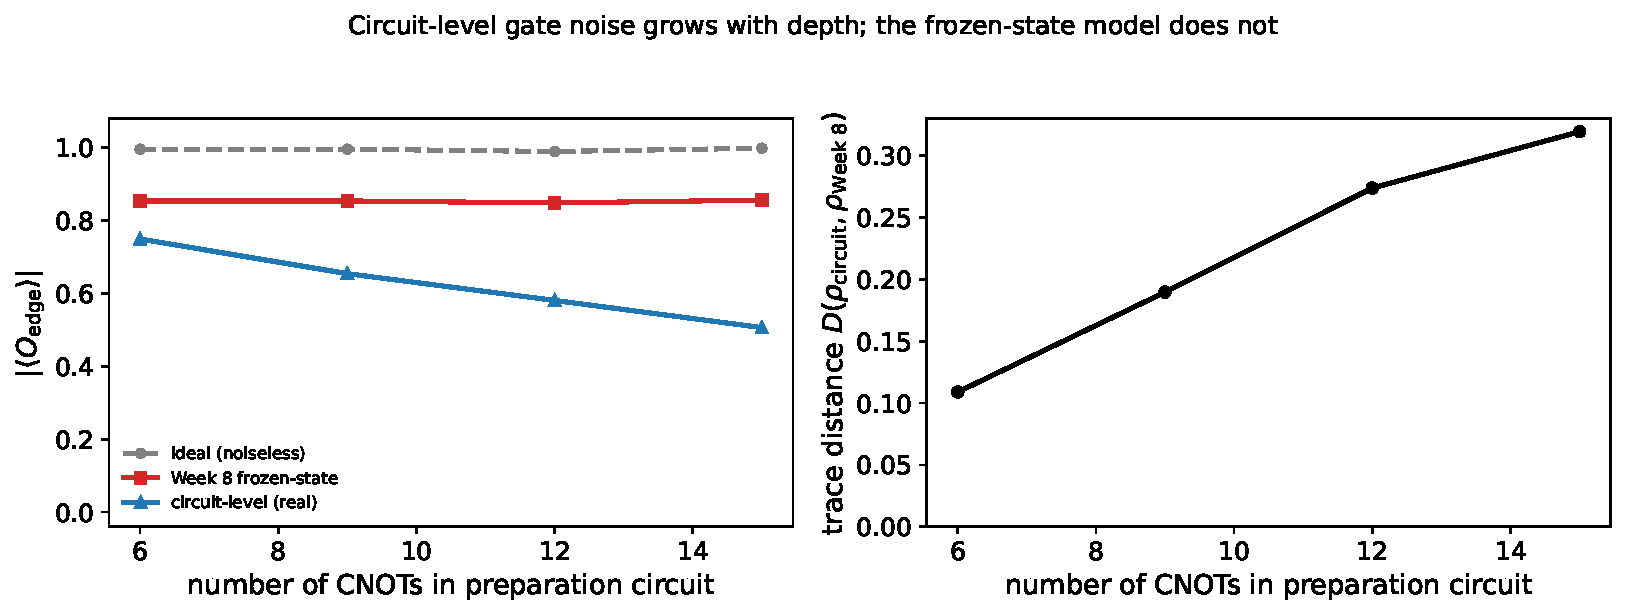
\includegraphics[width=\textwidth,height=0.78\textheight,keepaspectratio]{block4_week9_gate_noise.pdf}
    \end{column}
    \begin{column}{0.38\textwidth}
      \scriptsize
      Same $\theta$, matched per-channel strength ($\mu=0$):
      \begin{center}
      \begin{tabular}{cccc}
        \toprule
        CNOTs & circ. & W8 & $D$ \\
        \midrule
        6  & 0.75 & 0.85 & 0.11 \\
        9  & 0.66 & 0.85 & 0.19 \\
        12 & 0.58 & 0.85 & 0.27 \\
        15 & 0.51 & 0.86 & 0.32 \\
        \bottomrule
      \end{tabular}
      \end{center}
      \normalsize
      Week 8 stays \emph{flat}; the real circuit \emph{decays}. At depth 5 it over-estimates the signal by $\sim 70\%$.
    \end{column}
  \end{columns}
\end{frame}

\begin{frame}{Verification Across the Sweep + Topological Protection}
  \centering
  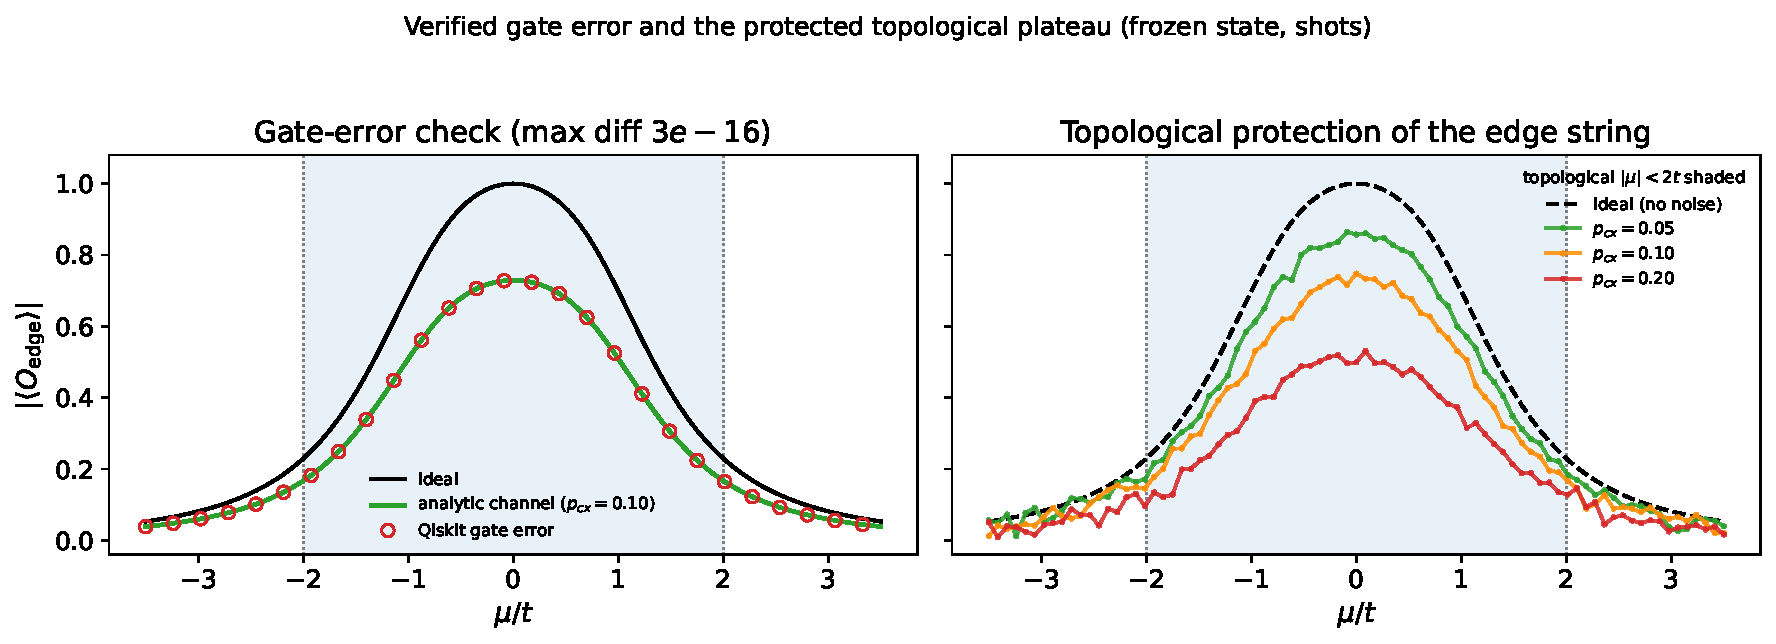
\includegraphics[width=0.98\textwidth,height=0.66\textheight,keepaspectratio]{block4_week9_topology_protection.pdf}

  \vspace{0.1cm}
  \footnotesize
  \textbf{Left:} analytic channel (line) vs Qiskit gate error (markers) agree to $3\times10^{-16}$ over all $\mu$.\quad
  \textbf{Right:} verified noise at three strengths; the topological plateau ($|\mu|<2t$) is suppressed but stays distinguishable from the trivial floor, most robustly at the $\mu=0$ sweet spot.
\end{frame}

\begin{frame}{What ``Topology Protects'' Means Here}
  \begin{itemize}
    \item The edge string measures the Majorana edge mode, which exists only for $|\mu|<2t$ and is protected there by the bulk gap.
    \item Under noise the topological signature is reduced in amplitude but not in \emph{location}: the phase distinction survives.
    \item The transitions $|\mu|=2t$ (gap closing) are the fragile points.
  \end{itemize}

  \begin{alertblock}{Careful statement}
    Decoherence is \emph{not} suppressed by topology -- without error correction, gate noise always lowers contrast. What the gap protects is the \emph{existence and localization} of the edge mode, so its signature remains measurable, most robustly deep in the topological phase.
  \end{alertblock}
\end{frame}

\begin{frame}{What This Enables Next}
  \begin{block}{Now that gate errors are integrated and verified}
    \begin{itemize}
      \item \textbf{Noisy VQE optimization}: optimize with a \texttt{NoiseModel}-backed estimator, so every cost evaluation is corrupted.
      \item \textbf{Backend-calibrated noise}: \texttt{NoiseModel.from\_backend(...)} for real device $T_1$/$T_2$ and gate errors.
      \item \textbf{Readout/SPAM layer}: fold the asymmetric assignment matrix into the same circuit-level model.
    \end{itemize}
  \end{block}
  \centering
  \footnotesize Full derivations and code: \texttt{notes/week9\_note.tex}, \texttt{src/block4.py} (plots 2--3).
\end{frame}

\end{document}
